\chapter{Verification test bed: high-lift configuration}
\label{cha_hlpw}
This chapter describes the remarkable results that our software and simulation methodology achieved while participating in the 3rd AIAA High-Lift Prediction Workshop, held in Denver, USA on June 3rd-4th, 2017 and serves as an introduction to Paper 1.
In the broader context of this thesis, the results described in this chapter serve as a validation of the methodology presented in Chapter~\ref{cha_adaptiveCFD}.

The workshop's goal was to assess the status of current CFD simulation technologies, and in particular their ability to simulate a high-lift aeroplane configuration, which represents the configuration of an aeroplane at take-off and landing.
This is all but a trivial problem: the main challenge today in CFD for aerodynamics is the ability to predict turbulent and separated flows.
The simulation of a full aircraft, as opposed to that of a more traditional wing profile, is even more challenging because the increased size of the computational domain increases the computational cost many times.
Typical engineering studies only focus on wing profiles, the main devices for lift generation, and currently DNS simulations at realistic Reynolds numbers are only barely possible for domains consisting of thin wing slices, and at an enormous computational cost; time-dependent LES and DNS simulations of a full aircraft are still a long way to come.

\section{Problem description}
\label{sec_problem}
The proposed benchmark is the simulation of flow past an aircraft model developed by the Japanese Aerospace Exploration Agency (JAXA) known as the JAXA Standard Model, or JSM, at a realistic Reynolds number of around \num{1.93e8}.
Figure~\ref{fig_hlpw_jsm} shows the wind tunnel setup that provided reference data for the benchmark.
\begin{wrapfloat}{figure}{O}{0pt}
  \centering
    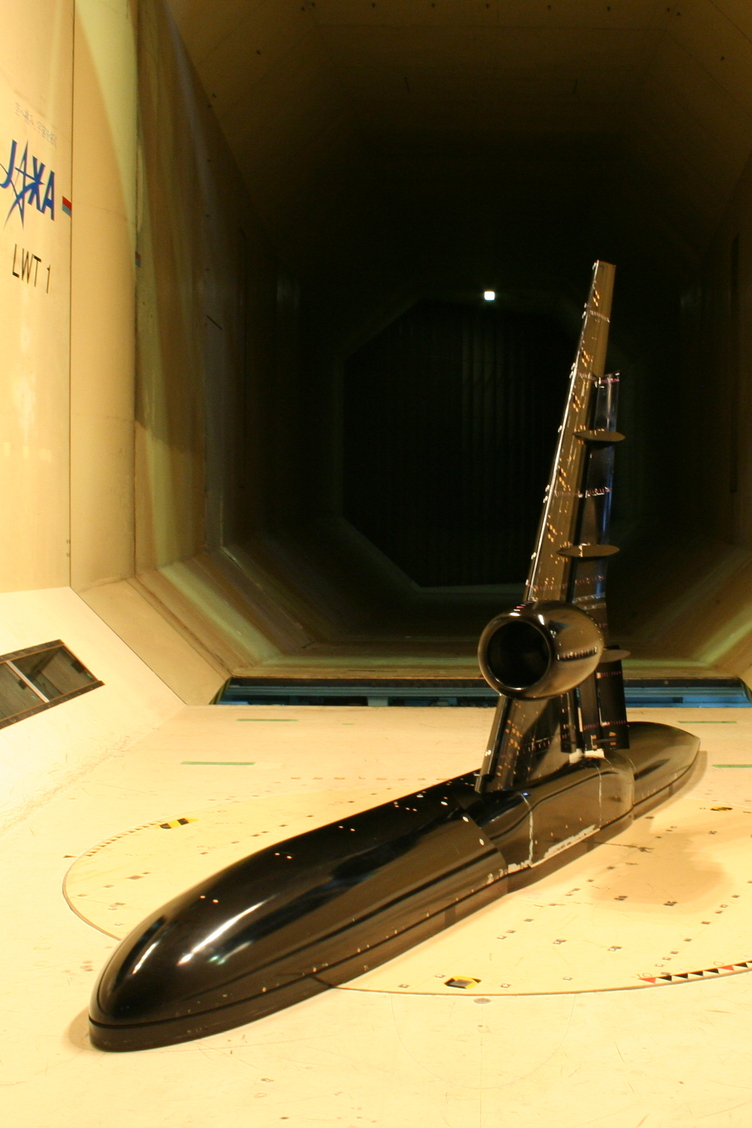
\includegraphics[width=0.5\columnwidth]{img/hlpw/jsm}
    \caption{A model of the JSM aeroplane in a wind tunnel.}
    \label{fig_hlpw_jsm}
\end{wrapfloat}
The main challenges in the simulation are the computation of drag and lift, with particular concern for the critical stall mechanism.
Lift generation tends to increase with increased angles of attack of a wing.
However, for a big enough angle of attack, the process abruptly interrupts and wings stop generating lift;
this phenomenon is called stall and should be avoided as it makes the aeroplane unable to fly, possibly with dramatic consequences.
For this reason, we had access to experimental results at a number of angle of attacks, from low values that are at no risk of stall to high values that exhibit stall.
The challenge is, of course, to simulate stall at the correct angle of attack.

The workshop proposed two configurations of the JSM for simulation, one with a nacelle (the \emph{pylon on} case) and one without a nacelle.
Given the small difference in reference aerodynamic forces given by experiments in the two cases, a difference of about \SI{2}{\percent}, we only focused on the \emph{pylon on} test case, which is the most complex and realistic of the two.

The organisers invited participants to test on two given meshes, a fine one to use as is and a coarser one to use with mesh adaptivity techniques.
Since the method we develop uses mesh adaptivity, we opted for the second approach, but we still generated our own mesh from the provided CAD files because the given mesh was not coarse enough.
It is worth pointing out at this point that our methodology can use a very coarse mesh as an initial mesh, the only requirement being that the geometric description of the surfaces, in this case of the aeroplane, be good enough to capture the geometric features.
The reason for this is that adaptive refinement near the surface does not improve the surface description in the sense that new points are not projected on the CAD shape from which the mesh was generated, as no CAD information is kept in the mesh.
Apart from this constraint, however, the volume mesh can be very coarse and the adaptive refinement will take care of adding mesh points where needed.
In particular, no specialised meshing knowledge is needed, nor any a priori knowledge of the features of the solution.

\section{Numerical tripping}
\label{sec_tripping}
The simulation of the stall cases was more challenging than the rest.
This is because stall is, from a physical point of view, generated by flow separation, in particular at the wing tip and near the wing-body junction, that detaches the flow and negatively affects the generation of lift.
The flow fields for the non-stalling configurations, which are well attached to the wing, are somewhat easier to reproduce; the transition to turbulence and consequent separation, on the other hand, were not.
We noted, in our first attempts, that the flow was not separating as expected.
Something similar happens with other numerical methods and the reason is that the inflow field, that is usually taken to be constant, is \emph{too perfect} to accurately represent reality.
In other words, no experiment in any wind tunnel will ever have a perfectly uniform and constant inflow, as is the case in numerical simulations, but rather an already chaotic inflow coming from air recirculation through the wind tunnel itself.
This means that the simulation would need a very long startup time to allow for numerical errors, the digital equivalent of physical perturbations, to grow and propagate in the flow field and reproduce a similar behaviour.

In the literature, an effective workaround is to add a small white-noise volume source term to the equation that has the effect of simulating this random perturbation in the inflow field.
In an attempt to strike a balance between a term that goes unnoticed and one that dominates over other effects, we scaled the white noise by \SI{5}{\percent} of the maximum of the pressure gradient.
We called this method \emph{numerical tripping} of the solution.

\section{Results overview}
\label{sec_results}
I will not go into the detailed results analysis for the test case, which is reported in the attached paper, but rather give an overview of the results and discuss their significance.

We performed simulations for a number of angles of attack in the range \((4, 23)\) starting from an initial mesh of just around \num{2.5e6} vertexes.
Unlike the experiment, which was performed on a half aeroplane profile, we created a mesh of a full profile to avoid modelling error introduced by a symmetry wall.
Figure~\ref{fig_hlpw_mesh} shows the surface mesh on the aeroplane geometry that we created, with Figure~\ref{fig_hlpw_meshDetail} showing the finest bits where the geometry is more complex.
\begin{figure}
  \centering
  \subfloat[][Surface mesh\label{fig_hlpw_meshAll}]
  {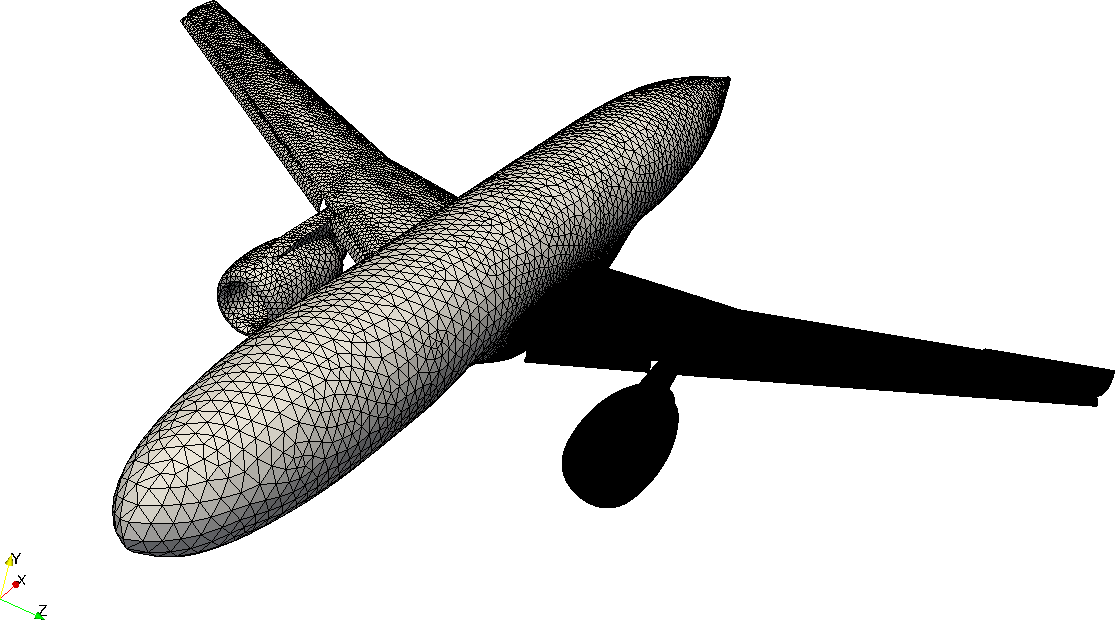
\includegraphics[width=0.45\textwidth]{img/hlpw/mesh}}
  \quad
  \subfloat[][Detail of wing mesh\label{fig_hlpw_meshDetail}]
  {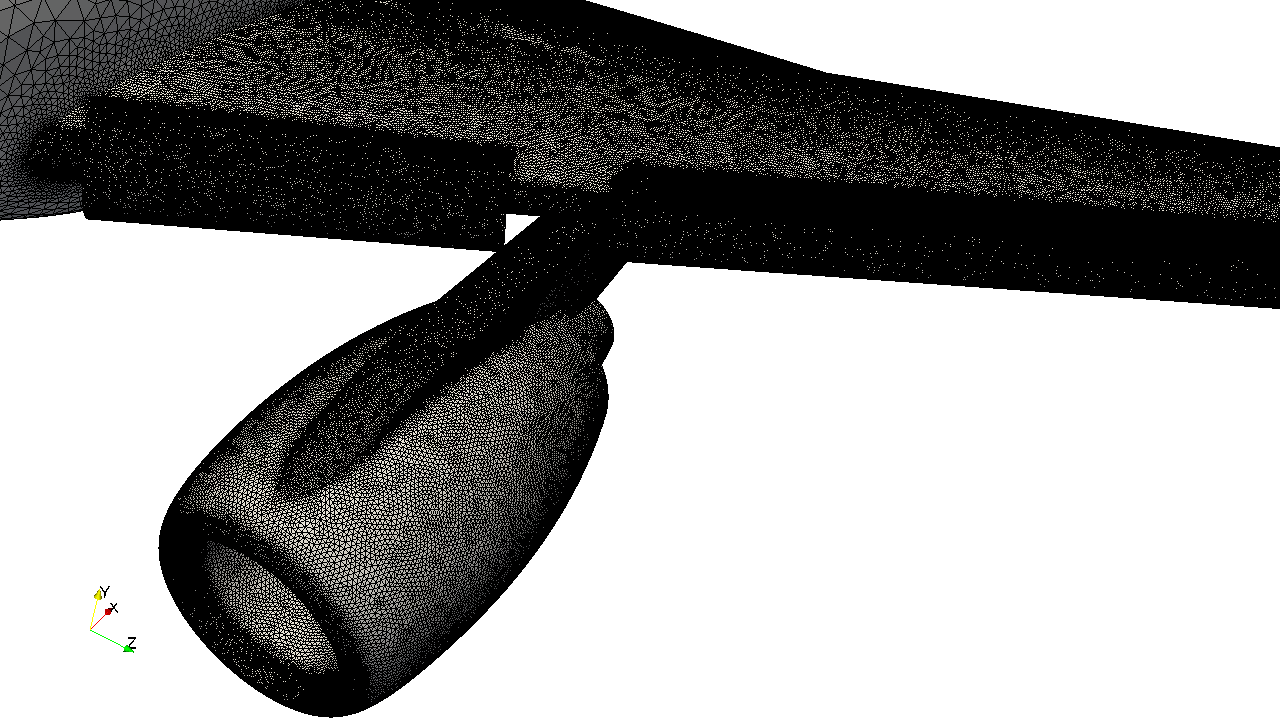
\includegraphics[width=0.45\textwidth]{img/hlpw/meshDetail}}
  \caption{The surface mesh we generated (left) and a detail of the mesh on the wing (right).}
  \label{fig_hlpw_mesh}
\end{figure}


Our starting mesh is significantly coarser than the provided one and allows for very cheap simulations.
At the end of our adaptive simulations, in which at each iteration we refined \SI{5}{\percent} of the cells, the finest meshes we had counted only \num{5e6} to \num{1e7} vertexes; for comparison, the tetrahedral mesh provided by the workshop had around \num{2.1e7} vertexes, meaning that even on our final runs we spent between a half and a fourth of the cost of running on the provided mesh.

We observed mesh convergence to experimental data for the lift coefficient within \SI{5}{\percent} for all the cases we ran, with a slightly bigger error of about \SI{10}{\percent} for the drag coefficient.
This is no surprise as the drag is notoriously more noisy and the typical drag signal oscillates noticeably, significantly more than the lift signal.

More importantly, for the configurations for which a stall is expected we were able to qualitatively simulate the stall mechanism, represented by a sharp drop in the lift force, for an angle of attack which differs from the experimental one by about \SI{1}{\degree}.

This is the most important feature of our results, and a remarkable achievement: our simulations were the only one to be time dependent, feature adaptivity and solve the full Navier-Stokes equations, and with the combination of these features we were able to both predict aerodynamic forces to values within experimental ranges and reproduce the correct physical separation in the flow field.
I would like to point out that nowhere in the code do we specify that we are interested in the separation, but we only ask for drag and lift.
The correct prediction of separation, together with the pressure profiles and other local quantities are simply a by-product of the method, that we were still able to recover without explicitly asking for them.

As an example, consider the visualisation in Figure~\ref{fig_hlpw_oil}, where experimental data from surface oil flow visualisation is compared to our simulation results.
\begin{figure}
  \centering
  \subfloat[][\(\alpha = 10.48^\circ\)\label{fig_hlpw_pylon_10_48_exp}]
  {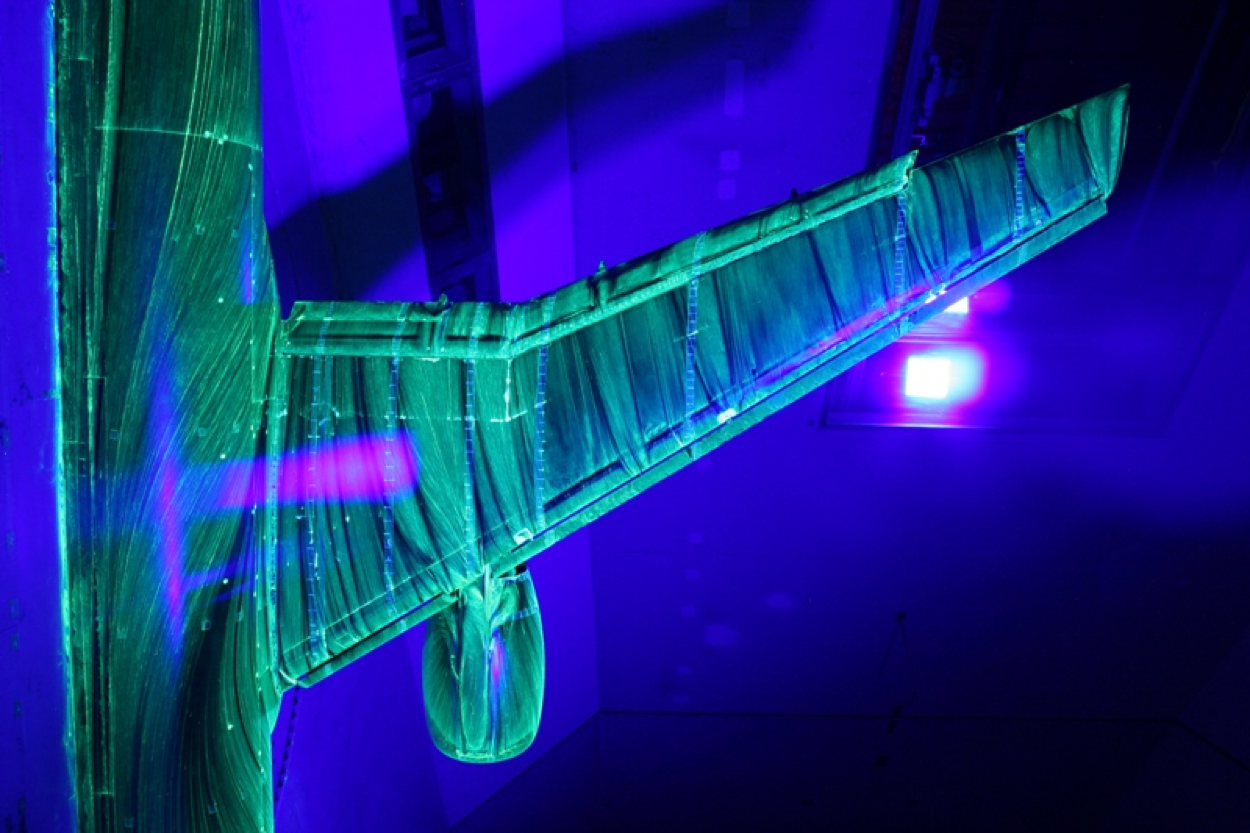
\includegraphics[width=0.45\textwidth]{img/hlpw/pylon_10_48_exp}}
  \quad
  \subfloat[][\(\alpha = 10.48^\circ\)\label{fig_hlpw_pylon_10_48_sim}]
  {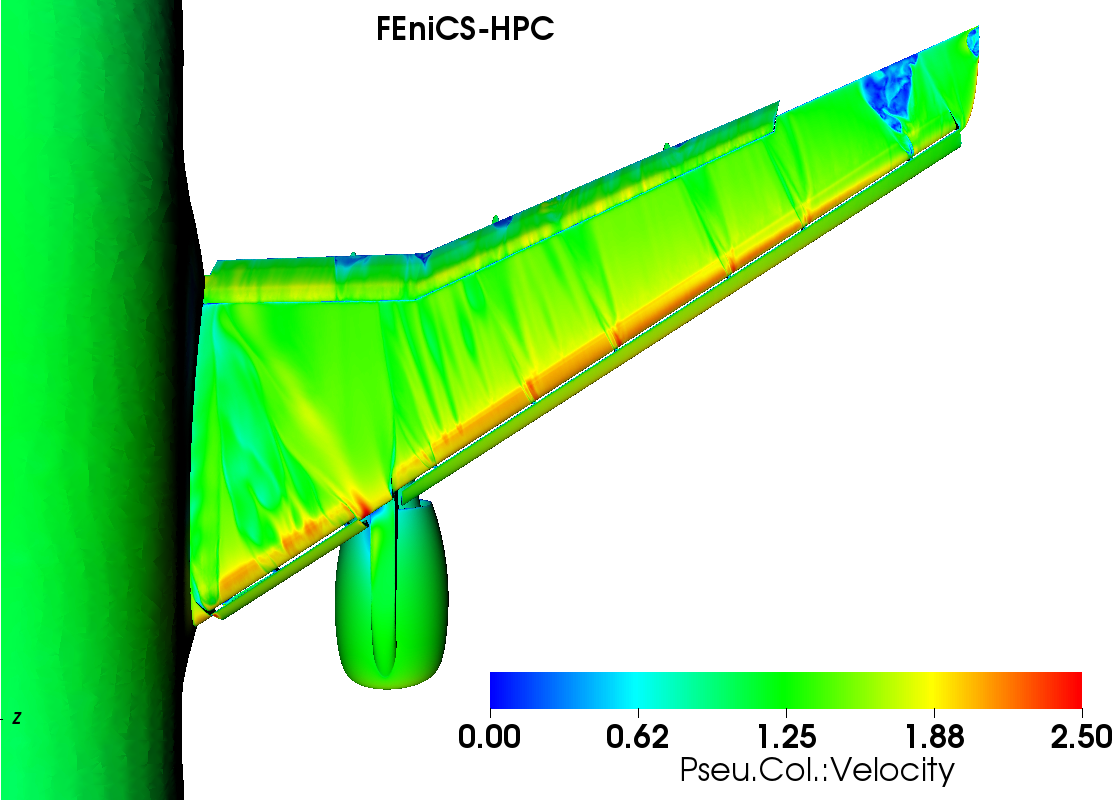
\includegraphics[width=0.45\textwidth]{img/hlpw/pylon_10_48_sim}}
  \\
  \subfloat[][\(\alpha = 18.58^\circ\)\label{fig_hlpw_pylon_18_58_exp}]
  {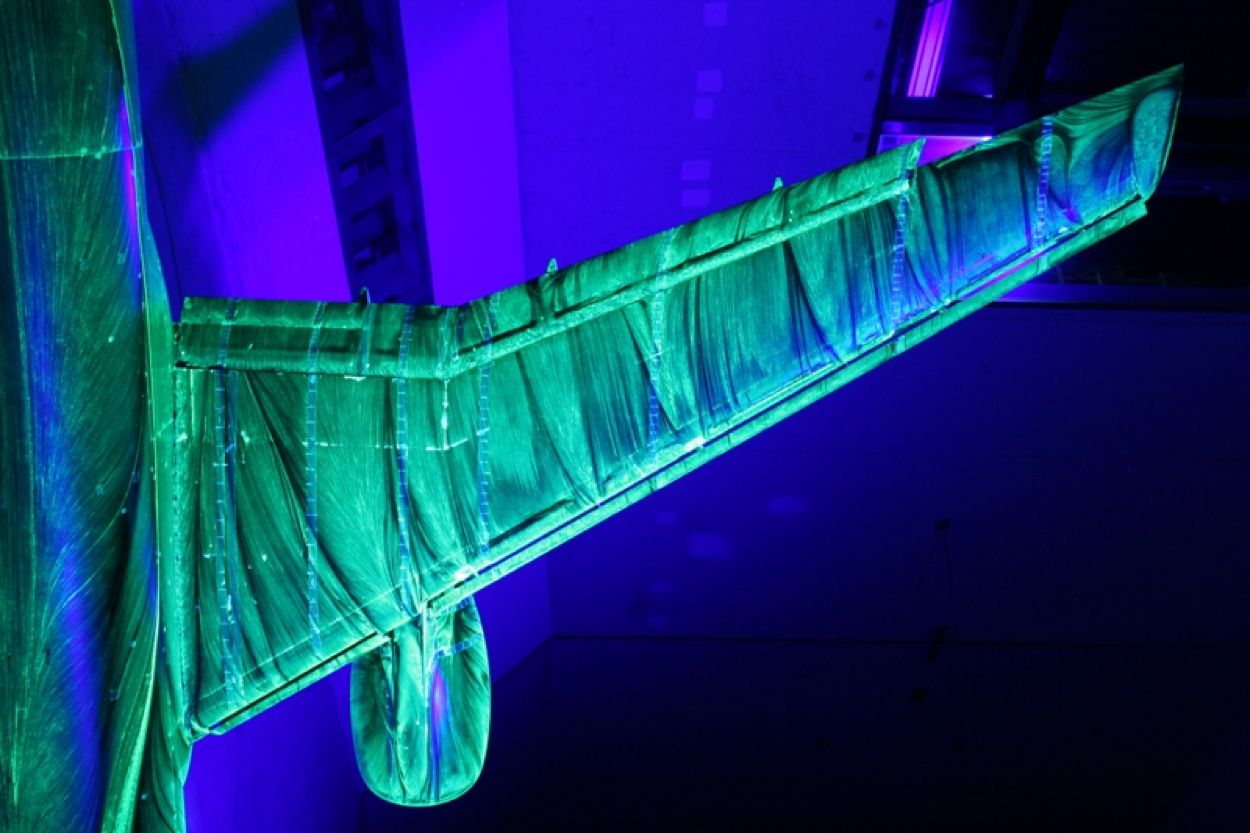
\includegraphics[width=0.45\textwidth]{img/hlpw/pylon_18_58_exp}}
  \quad
  \subfloat[][\(\alpha = 18.58^\circ\)\label{fig_hlpw_pylon_18_58_sim}]
  {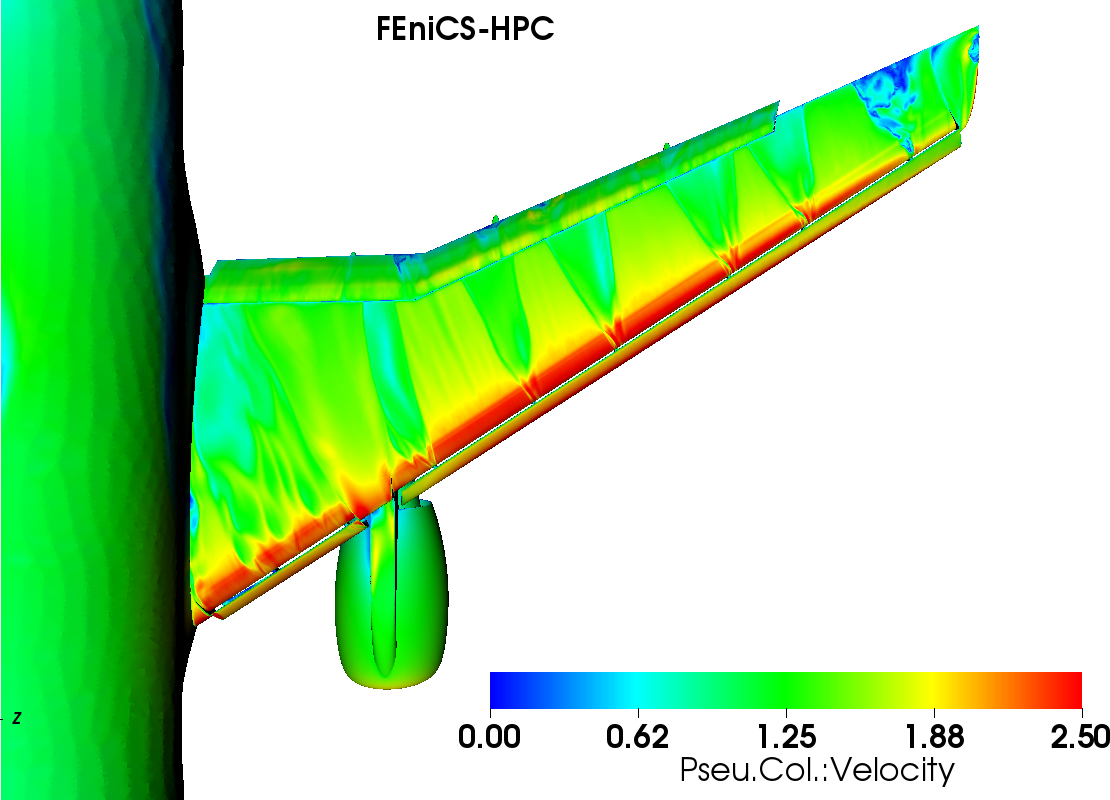
\includegraphics[width=0.45\textwidth]{img/hlpw/pylon_18_58_sim}}
  \\
  \subfloat[][\(\alpha = 21.57^\circ\)\label{fig_hlpw_pylon_21_57_exp}]
  {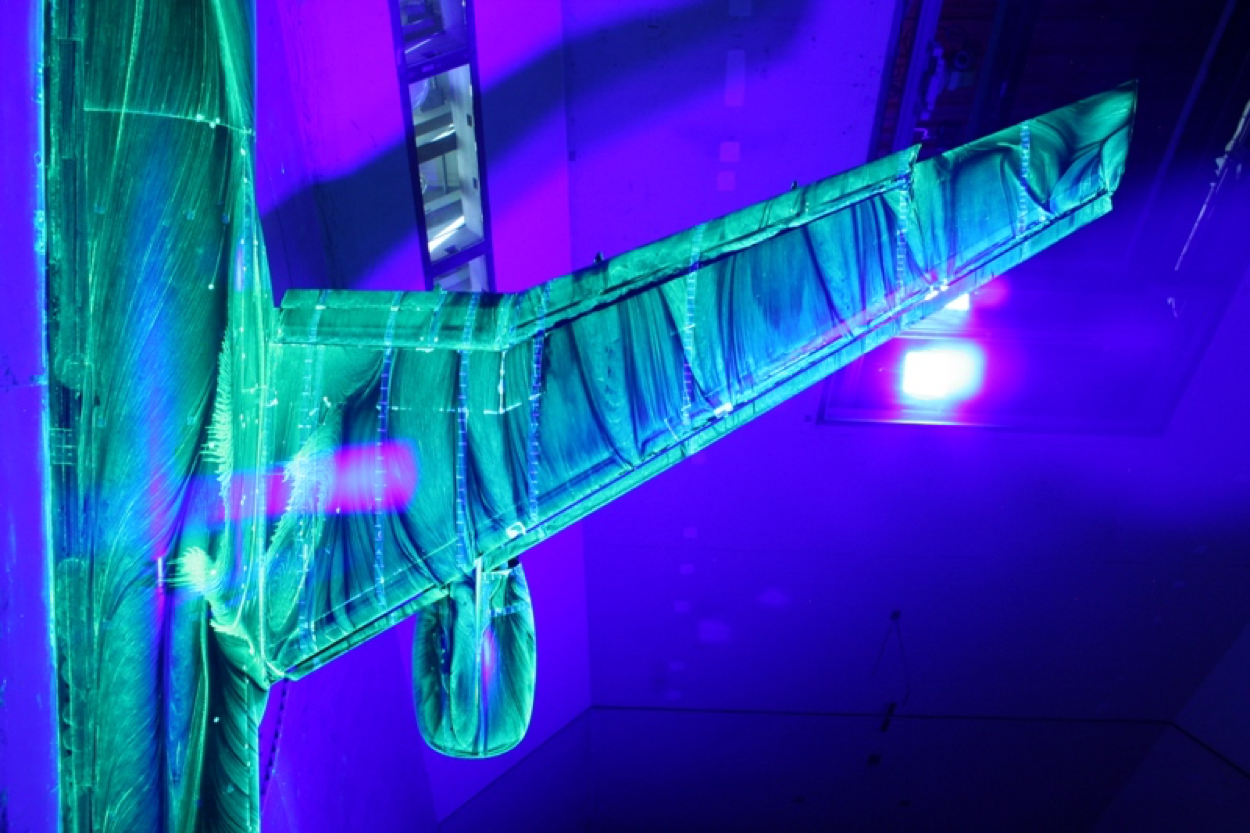
\includegraphics[width=0.45\textwidth]{img/hlpw/pylon_21_57_exp}}
  \quad
  \subfloat[][\(\alpha = 22.56^\circ\)\label{fig_hlpw_pylon_22_56_sim}]
  {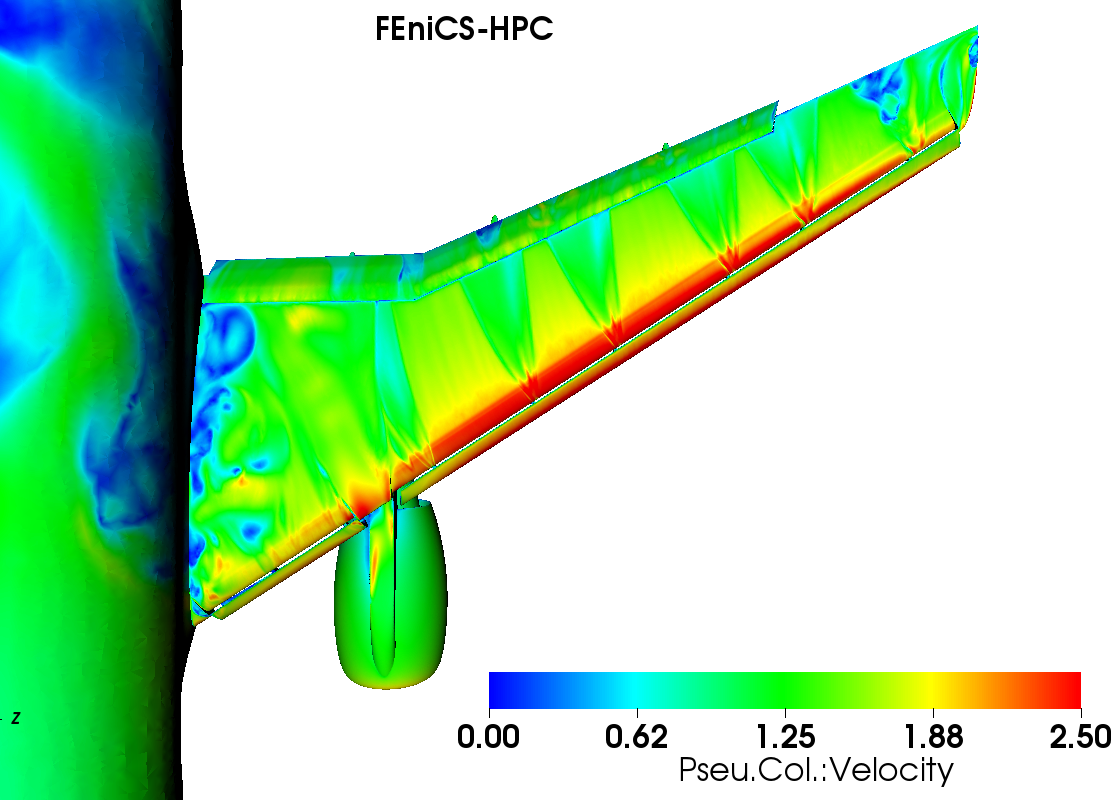
\includegraphics[width=0.45\textwidth]{img/hlpw/pylon_22_56_sim}}
  \\
  \caption{Comparison of surface oil flow visualisation from the wind tunnel and velocity profiles from our simulations.}
  \label{fig_hlpw_oil}
\end{figure}
What should be noticed in Figure~\ref{fig_hlpw_oil} is that the simulation results closely match the profiles in the experimental setup, in particular the V-shaped structures originating from where the leading edge of the wing is connected to the flaps.
In the first two rows the flow is attached as we are not at the stall angle yet, but the third row shows an important additional feature: separation at the wing-body junction, visually denoted by the blue, low velocity area on the left of Figure~\ref{fig_hlpw_pylon_22_56_sim}.

To give another point of view on the same phenomenon, Figure~\ref{fig_hlpw_pylon_22_56_vorticity} visualises the separation via the vorticity in the volume.\begin{figure}
  \centering
    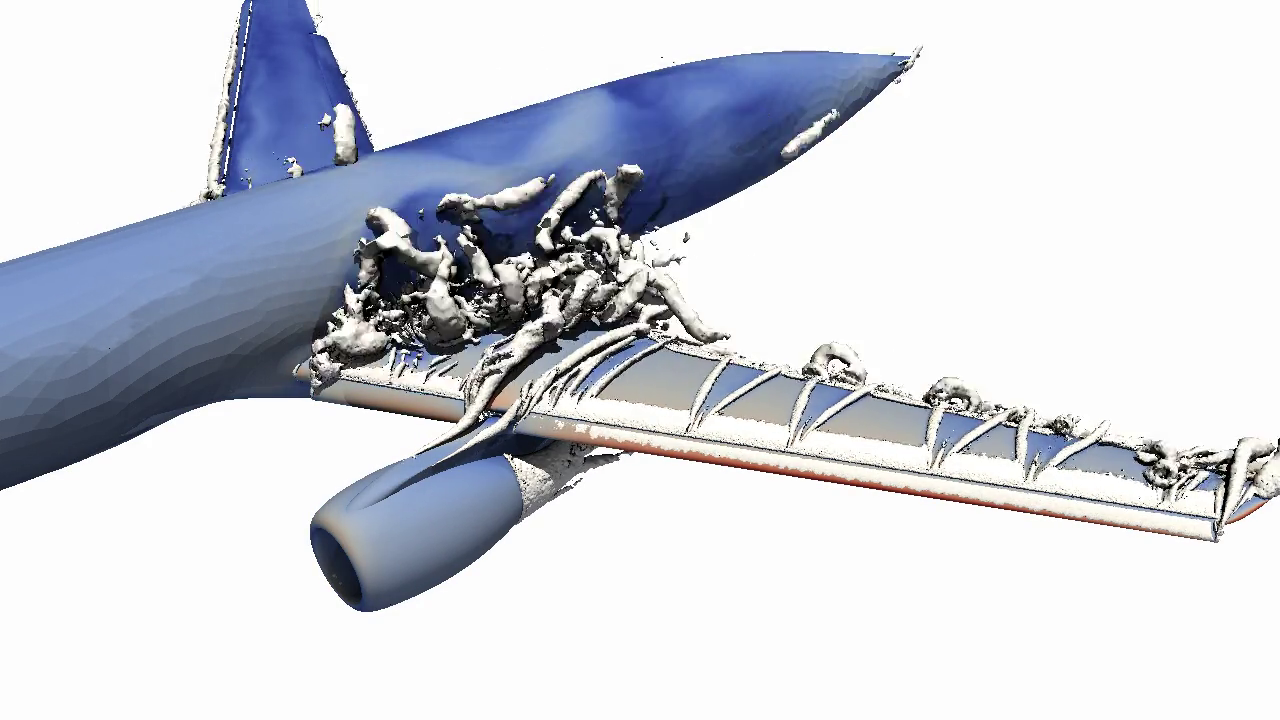
\includegraphics[width=\columnwidth]{img/hlpw/pylon_22_56_vorticity}
    \caption{Visualisation of turbulent separation via vorticity computed with the Q-criterion.}
    \label{fig_hlpw_pylon_22_56_vorticity}
\end{figure}
It represents a snapshot of a fully-developed flow field, showing how the turbulent separation grows from the wing-body junction

Again, I think it is worth pointing out that the code was not tuned to resolve the separation, but only the aerodynamic forces; the rest is a by-product of the method that naturally resolves the correct physical mechanisms at play, in this case stall.
